\documentclass[../main.tex]{subfiles}
\usepackage{../style}
\graphicspath{ {../img/} }
\begin{document}
\chapter{De Broglie Waves (Matter Waves)}
In 1924, Lewis de-Broglie proposed that matter has dual nature just like photon. His concept about the dual nature of matter was based on the following observations:
\begin{itemize}
    \item The whole universe is composed of matter and electromagnetic radiations. Since both are forms of energy so can be transformed into each other.
    \item The nature loves symmetry. As  the radiation has dual nature, matter should also possess dual character.
\end{itemize}
According to the de Broglie concept of matter waves the matter has dual nature. It means when the matter is moving it shows the wave properties are associated with it and when it is at rest then it shows particle properties. Thus, the matter has dual nature. The waves associated with moving particles are called matter waves or de-Broglie waves.
\section{De Broglie Wave Length}
The energy of a photon can be written as $ E=hv=\frac{hc}{\lambda} $, if a photon possess mass (rest mass is zero), then according to the theory of relativity its energy is given by,
\[
    E=mc^2=mc\cdot c=pc
\]
Hence the momentum of a photon
\[
    p=\frac{E}{c}=\frac{hc}{\lambda c}=\frac{h}{\lambda}
\]
wavelength of a photon, 
\[
    \lambda=\frac{h}{p}
\]
Instead of photon, we consider a particle of mass $ m $ moving with velocity $ v $, then the momentum of the particle $ p=mv $ then wavelength of that particle will be
\[
    \boxed{\lambda=\frac{h}{mv}} \longrightarrow \text{de-Broglie wavelength}
\]
where, $\displaystyle m=\frac{m_0}{\sqrt{1-v^2/c^2}} $, the relativistic mass.
\section{Phase Velocity and Group Velocity}
According to de-Broglie's concept of matter waves, each particle of matter (like electron, proton etc) while in potion, may be regarded as consisting of a group of waves or a wave packet as it is called the wave packet, formed by superposition of a number of waves and traveling with the velocity of the particles, behaves very much like a corpuscle. Each component wave propagates with a definite velocity called the wave velocity or phase velocity. But when a disturbance consists of a number of component waves, each travelling with slightly different velocity, the resultant velocity will be that of a periodicity. The velocity with which the periodicity advances is called the Group velocity.
\subsection{Derivation of the formula of phase and group velocity}
Let us consider that the wave group arises from the combination of two waves that have the same amplitude. A bit differs by an amount $ \Delta\, \omega $ in angular frequency and an amount $ \Delta\, k $ in wave number. We may suspect the original waves by the formulas,
\begin{align*}
    y_1&=A\cos(\omega\,t-kx)\\
    y_2&=A\cos\left[ (\omega+\Delta\, \omega)t-(k+\Delta\, k)x \right]
\end{align*}
The resultant displacement $ y $ at time $ t $ and any position $ x $ is the sum of $ y_1 $ and $ y_2 $.
\begin{figure}[ht]
    \centering
    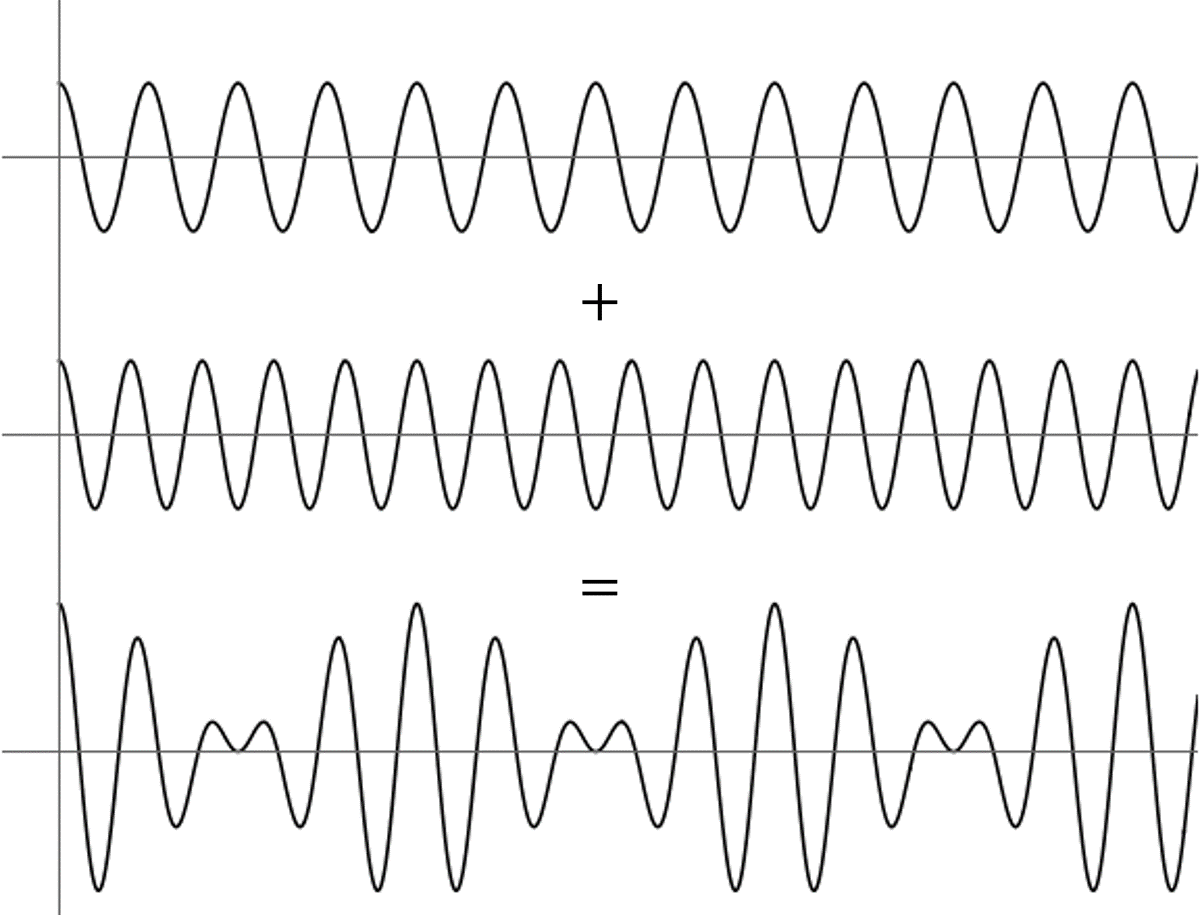
\includegraphics[scale=.5]{de-Broglie-wave-derivation.png}
\end{figure}
\begin{align*}
    y&=y_1+y_2\\
    &=A\cos(\omega \,t-kx)+A\cos\left[ (\omega+\Delta\, \omega)t-(k+\Delta\, k)x \right]\\
    &=2A\cos\frac{\omega\,t-kx+\omega\,t+\Delta\, \omega\, t-kx-\Delta\, kx}{2}\cdot \cos\frac{\omega\,t-kx-\omega\,t-\Delta\, \omega t+kx+\Delta\, kx}{2}\\
    &=2A\cos\frac{1}{2}\left[ (2x+\Delta\, \omega)t-(2k+\Delta\, k)x \right]\times \cos\frac{1}{2}\left( \Delta\, \omega\,t-\Delta\, kx \right)
\end{align*}
Since $ \Delta\, \omega $ and $ \Delta\, k $ are small compared with $ \omega $ and $ k $.
\[
    2\omega+\Delta\, \omega\approx 2\omega\qquad \text{and}\qquad 2k+\Delta\, k=2k
\]
So,
\[
    y=2A \cos\left( \omega\,t-kx \right)\cdot\cos\left( \frac{\Delta\, \omega}{2}t-\frac{\Delta\, k}{2}x \right)
\]
This equation represent a wave of angular frequency $ \omega $ and wave number $ k $ that has superimposed upon it a modulation of angular frequency $ \frac{1}{2}\Delta\, \omega $ and of wave number $ \frac{1}{2}\Delta\, k $.

The effect of the modulation is thus to produce successive wave group. The phase velocity, $ v_p $ is,
\[\boxed{v_p=\frac{\omega}{k}}\longrightarrow\text{Phase Velocity}\]
and the group velocity, $ v_g $ is,
\[\boxed{v_g=\frac{\Delta\,\omega}{\Delta\,k}}\longrightarrow\text{Group Velocity}\]
when $\omega $ and $ k $ have continuous speeds then,
\[\boxed{v_g=\frac{\D \omega}{\D k}}\]
Depending on how phase velocity varies with wave number in a particular situation, the group velocity may greater or less than the phase velocities of its member waves.

The angular frequency and wave number of the de-Broglie waves associated with a body at rest mass $ m_0 $ moving with velocity $ v $ are,
\[
    \omega=2\pi v=\frac{2\pi m c^2}{h}
\]
high frequency of de-Broglie waves,
\[\omega=\frac{2\pi m_0 c^2}{h\sqrt{1-v^2/c^2}}\]
Both $ \omega $ and $ k $ are functions of the body's velocity $ v $.\\
The group velocity $ v_g $ of the de-Broglie waves associated with body is,
\[v_g=\frac{\D\omega }{\D k}=\frac{\displaystyle\frac{\D \omega}{\D v}}{\displaystyle\frac{\D k}{\D v}}\left\vert\begin{aligned}
    \frac{\D\omega}{\D v}&=\frac{2\pi m_0v}{h\left( 1-\frac{v^2}{c^2} \right)^\frac{3}{2}}\\
    \frac{\D k}{\D v}&=\frac{2\pi m_0}{h\left( 1-\frac{v^2}{c^2} \right)^\frac{3}{2}}
\end{aligned}\right.\]
De Broglie group velocity
\[\boxed{v_g=v}\]
The de Broglie wave group associated with moving body travels with the same velocity as the body,
\[\boxed{v_p=\frac{\omega}{k}=\frac{c^2}{v}}\longrightarrow\text{De Broglie Phase Velocity}\]
\begin{prob}
    An electron has a de Broglie wavelength of $ 2 pm $. Find its kinetic energy and the phase and group velocities of its de-Broglie waves. [The rest energy of electron$ =511KeV $]
\end{prob}
\begin{soln}
    \begin{align*}
        pc&=\frac{hc}{A}=\frac{\left( 4.13\E{-15} \right)\left( 3\E{8} \right)}{2\E{-12}}\\
        &=6.20\E{5}eV\\
        &=620KeV
    \end{align*}
    Now,
    \begin{align*}
        KE&=E-E_0\\
        &=\sqrt{E_0^2+\left( pc \right)^2}-E_0\\
        &=\sqrt{(511)^2+\left( 620 \right)^2}-511\\
        &=292KeV
    \end{align*}
    The electron velocity can be found from
    \begin{align*}
        E&=\frac{E_0}{\sqrt{1-v^2/c^2}}\\
        \Rightarrow\,v&=c\sqrt{1-E_0^2/E^2}\\
        \Rightarrow\,v&=c\sqrt{1-\frac{511^2}{803^2}}\\
        &=0.771c
    \end{align*}
    Hence,
    \begin{align*}
        \text{the group velocity, } v_g&=v=0.771c\\
        \text{the phase velocity, } v_p&=\frac{c^2}{v}=1.30c
    \end{align*}
\end{soln}
\end{document}